% Overleaf			
%% Software Manual and Technical Document Template	
%% 									
%% This provides an example of a software manual created in Overleaf.

\documentclass{../ol-softwaremanual}

% Packages used in this example
\usepackage{graphicx}  % for including images
\usepackage{microtype} % for typographical enhancements
\usepackage{minted}    % for code listings
\usepackage{amsmath}   % for equations and mathematics
\setminted{style=friendly,fontsize=\small}
\renewcommand{\listoflistingscaption}{List of Code Listings}
\usepackage{hyperref}  % for hyperlinks
\usepackage[a4paper,top=4.2cm,bottom=4.2cm,left=3.5cm,right=3.5cm]{geometry} % for setting page size and margins

\usepackage[english, greek]{babel}

\usepackage{subfig}

\usepackage{longtable}


% Custom macros used in this example document
\newcommand{\doclink}[2]{\href{#1}{#2}\footnote{\url{#1}}}
\newcommand{\cs}[1]{\texttt{\textbackslash #1}}

\begin{document}
	
	
	\begin{titlepage}
		
		
		% Frontmatter data; appears on title page
		\title{\en Project Plan \\}
		\version{1.0}
		\softwarelogo{\includegraphics[scale=0.4]{../CarBazaar\_logo.png}}
	\end{titlepage}
	
	
	\maketitle
	
	\newpage
	
	\center{\textbf{Μέλη Ομάδας}}
	
	\vspace{20pt}
	
	
	
	\begin{table}[htbp!]
		
		\begin{tabular}{llll}
			Μεμελετζόγλου Χαρίλαος & 1069364 & \en st1069364@ceid.upatras.gr & 4o Έτος   \\ 
			\\ Λέκκας Γεώργιος      &      1067430    &   \en st1067430@ceid.upatras.gr & 4o Έτος  \\
			\\ Γιαννουλάκης Ανδρέας        &   1067387       & \en st1067387@ceid.upatras.gr & 4o Έτος           \\
			\\ Κανελλόπουλος Ιωακείμ        &  1070914        &    \en st1070914@ceid.upatras.gr & 4o Έτος        \\ 
		\end{tabular}
	\end{table}
	
	\center{\textbf{Υπεύθυνοι Παρόντος Τεχνικού Κειμένου}}
	
	\vspace{20pt}
	
	\begin{table}[htbp!]
		\begin{tabular}{ll}
			Μεμελετζόγλου Χαρίλαος & \en Editor \\
			\\ Λέκκας Γεώργιος      &   \en  Editor \\
			\\ Γιαννουλάκης Ανδρέας & \en Contributor \\
			\\ Κανελλόπουλος Ιωακείμ & \en Contributor \\ 
		\end{tabular}
	\end{table}
	
	\center{\textbf{Αλλαγές στην έκδοση \en v1.0 \gr}}
	\vspace{10pt}
	\flushleft
	
	Είναι η έκδοση \en \textbf{v0.2} \gr, χωρίς καμία αλλαγή.
	
	\vspace{20pt}
	
	\center{\textbf{Εργαλεία που χρησιμοποιήθηκαν}}
	
	
	\flushleft
	Χρησιμοποιήθηκε το \en \doclink{https://www.overleaf.com/}{Overleaf} \gr για την συγγραφή του \LaTeX\ κώδικα. \break
	
	Για την δημιουργία του λογότυπου, χρησιμοποιήθηκε το εργαλείο \en \doclink{https://www.adobe.com/express/create/logo}{Adobe Express} . \gr \break
	
	Για την ανάπτυξη του έργου χρησιμοποιείται η γλώσσα προγραμματισμού \en Python \gr και για την συγγραφή του κώδικα, το \en IDE \doclink{https://www.jetbrains.com/pycharm/}{PyCharm} \gr και το \en \doclink{https://code.visualstudio.com/}{VSCode} \gr .         \\ \break
	
	Για την δημιουργία του \en Gantt Chart, \gr χρησιμοποιήθηκε το \en \doclink{https://instagantt.com/}{Instagantt} \gr και για την δημιουργία του \en Pert Chart \gr, το \en \doclink{https://www.smartdraw.com/}{Smartdraw} \gr. \break 
	
	Για την παρακολούθηση των \en To-Do tasks \gr, των ολοκληρωμένων,κλπ, δηλ. για την δημιουργία ενός \en Scrum Board \gr, θα χρησιμοποιηθεί το \en site \doclink{https://trello.com/}{Trello} \gr. \break 
	
	Για την επικοινωνία των μελών της ομάδας, χρησιμοποιείται το \en \doclink{ https://www.discord.com/}{Discord} \gr . \linebreak 
	
	
	Για τον διαμοιρασμό και την παρακολούθηση της διαδικασίας ανάπτυξης, χρησιμοποιείται το \en \doclink{https://github.com/st1069364/CarBazaar}{Github} \gr.
	
	
	
	\newpage
	
	\center{\textbf{Υποθετικός μακροπρόθεσμος χρονοπρογραμματισμός του Έργου}}
	\flushleft
	
	\vspace{20pt}
	
	Έστω ότι η ομάδα μας αποφασίζει να συνεχίσει την ενασχόλησή της με το έργο και μετά το πέρας του εαρινού εξαμήνου. Καθώς θα προχωρήσουμε σε μία ολοκληρωμένη υλοποίηση του έργου, είναι λογικό πως τα \en tasks \gr που πρέπει να διεκπεραιωθούν, θα είναι περισσότερα σε σχέση με αυτά που υλοποιήθηκαν κατά την διάρκεια του εξαμηνιαίου έργου.
	
	\vspace{20pt}
	
	Τα \en tasks, \gr π.χ περισσότερα \en mockup screens\gr, επιλογή επιπλέον προγραμματιστικών εργαλείων,  χρονοδιάγραμμα για δοκιμές και ελέγχους λαθών, κλπ, αποτυπώνονται πάνω στα διαγράμματα \en Gantt \gr και \en Pert \gr μαζί με τις αντίστοιχες ημερομηνίες εφαρμογής τους. \break
	
	Για τα \en tasks \gr που φαίνονται στα παρακάτω \en Gantt \& Pert Charts \gr, έχουν χρησιμοποιηθεί ως πηγή έμπνευσης, οι ιστοσελίδες : 
	
	\begin{itemize}
		\item \en \url{https://www.invonto.com/insights/mobile-app-development-process/}
		\item \en \url{https://thebhwgroup.com/blog/mobile-app-development-process}
		\item \en \url{https://www.mindbowser.com/a-step-by-step-guide-to-mobile-app-development/}
	\end{itemize}
	\vspace{5pt}
	
	Ως ημερομηνία έναρξης του \en project \gr έχει οριστεί η 1η Μαρτίου και ως ημερομηνία λήξης έχουμε, 14/5/2022 . Θεωρούμε πως η ομάδα θα εργάζεται 6 μέρες την εβδομάδα, και πιθανόν να χρειαστούν και κάποιες υπερωρίες προκειμένου να παραδώσουμε στον πελάτη όσο πιο γρήγορα γίνεται το έργο. \\
	
	\newpage
	
	
	\center{\textbf{\en Gantt Chart \gr Έργου}}
	\vspace{10pt}	
	
	Παρακάτω παρατίθεται ο αρχικός χρονοπρογραμματισμός του έργου.
	
	\vspace{10pt}
	
	
	\flushleft
	
	\begin{figure}[htbp!]
		
		\includegraphics[width=\textwidth,height=\textheight,keepaspectratio]{img/gantt\_chart\_project\_plan.png}
		\caption{\en Gantt Chart \gr έργου}
		
		
	\end{figure}
	
	\vspace{20pt}
	Ορίζουμε τα εξής \en Milestones \gr :
	
	\begin{itemize}
		\item \en Milestone 1 : App Initial Version
		\item \en Milestone 2 : Backend Integrated w/ App
		\item \en Milestone 3 : Published Companion Website
		\item \en Milestone 4: Project End
	\end{itemize}
	
	
	\newpage 
	
	\center{\textbf{\en Pert Chart \gr Έργου}}
	\flushleft
	Παρακατω παρατίθεται το \en Pert Chart \gr, όπως αυτό προκύπτει από το αντίστοιχο \en Gantt Chart \gr και αποτυπώνει σχηματικά τα χρονικά πλαίσια ανάμεσα στα \en tasks\gr, αλλά και τις εξαρτήσεις που προκύπτουν κατά την διαδικασία ανάπτυξης του έργου, οι οποίες απεικονίζονται μέσω του \en Critical Path \gr, το οποίο απεικονίζεται μέσω κόκκινων ακμών.
	
	
	\begin{figure}[htbp!]
		
		\includegraphics[width=\textwidth, height=\textheight, keepaspectratio ]{img/PertChart\_for\_Projectplan.jpg}
		\caption{ \en Pert Chart \gr Έργου}
	\end{figure}
	
	\newpage
	
	\center{\textbf{ \en Gantt Chart \gr και Πίνακας ανάθεσης Έργου σε ανθρώπινο δυναμικό}}
	\vspace{20pt}
	\flushleft
	Στο παρακάτω \en Gantt Chart \gr πραγματοποιείται ανάθεση των \en tasks \gr στα μέλη της ομάδας.
	
	\begin{figure}[htbp!]
		
		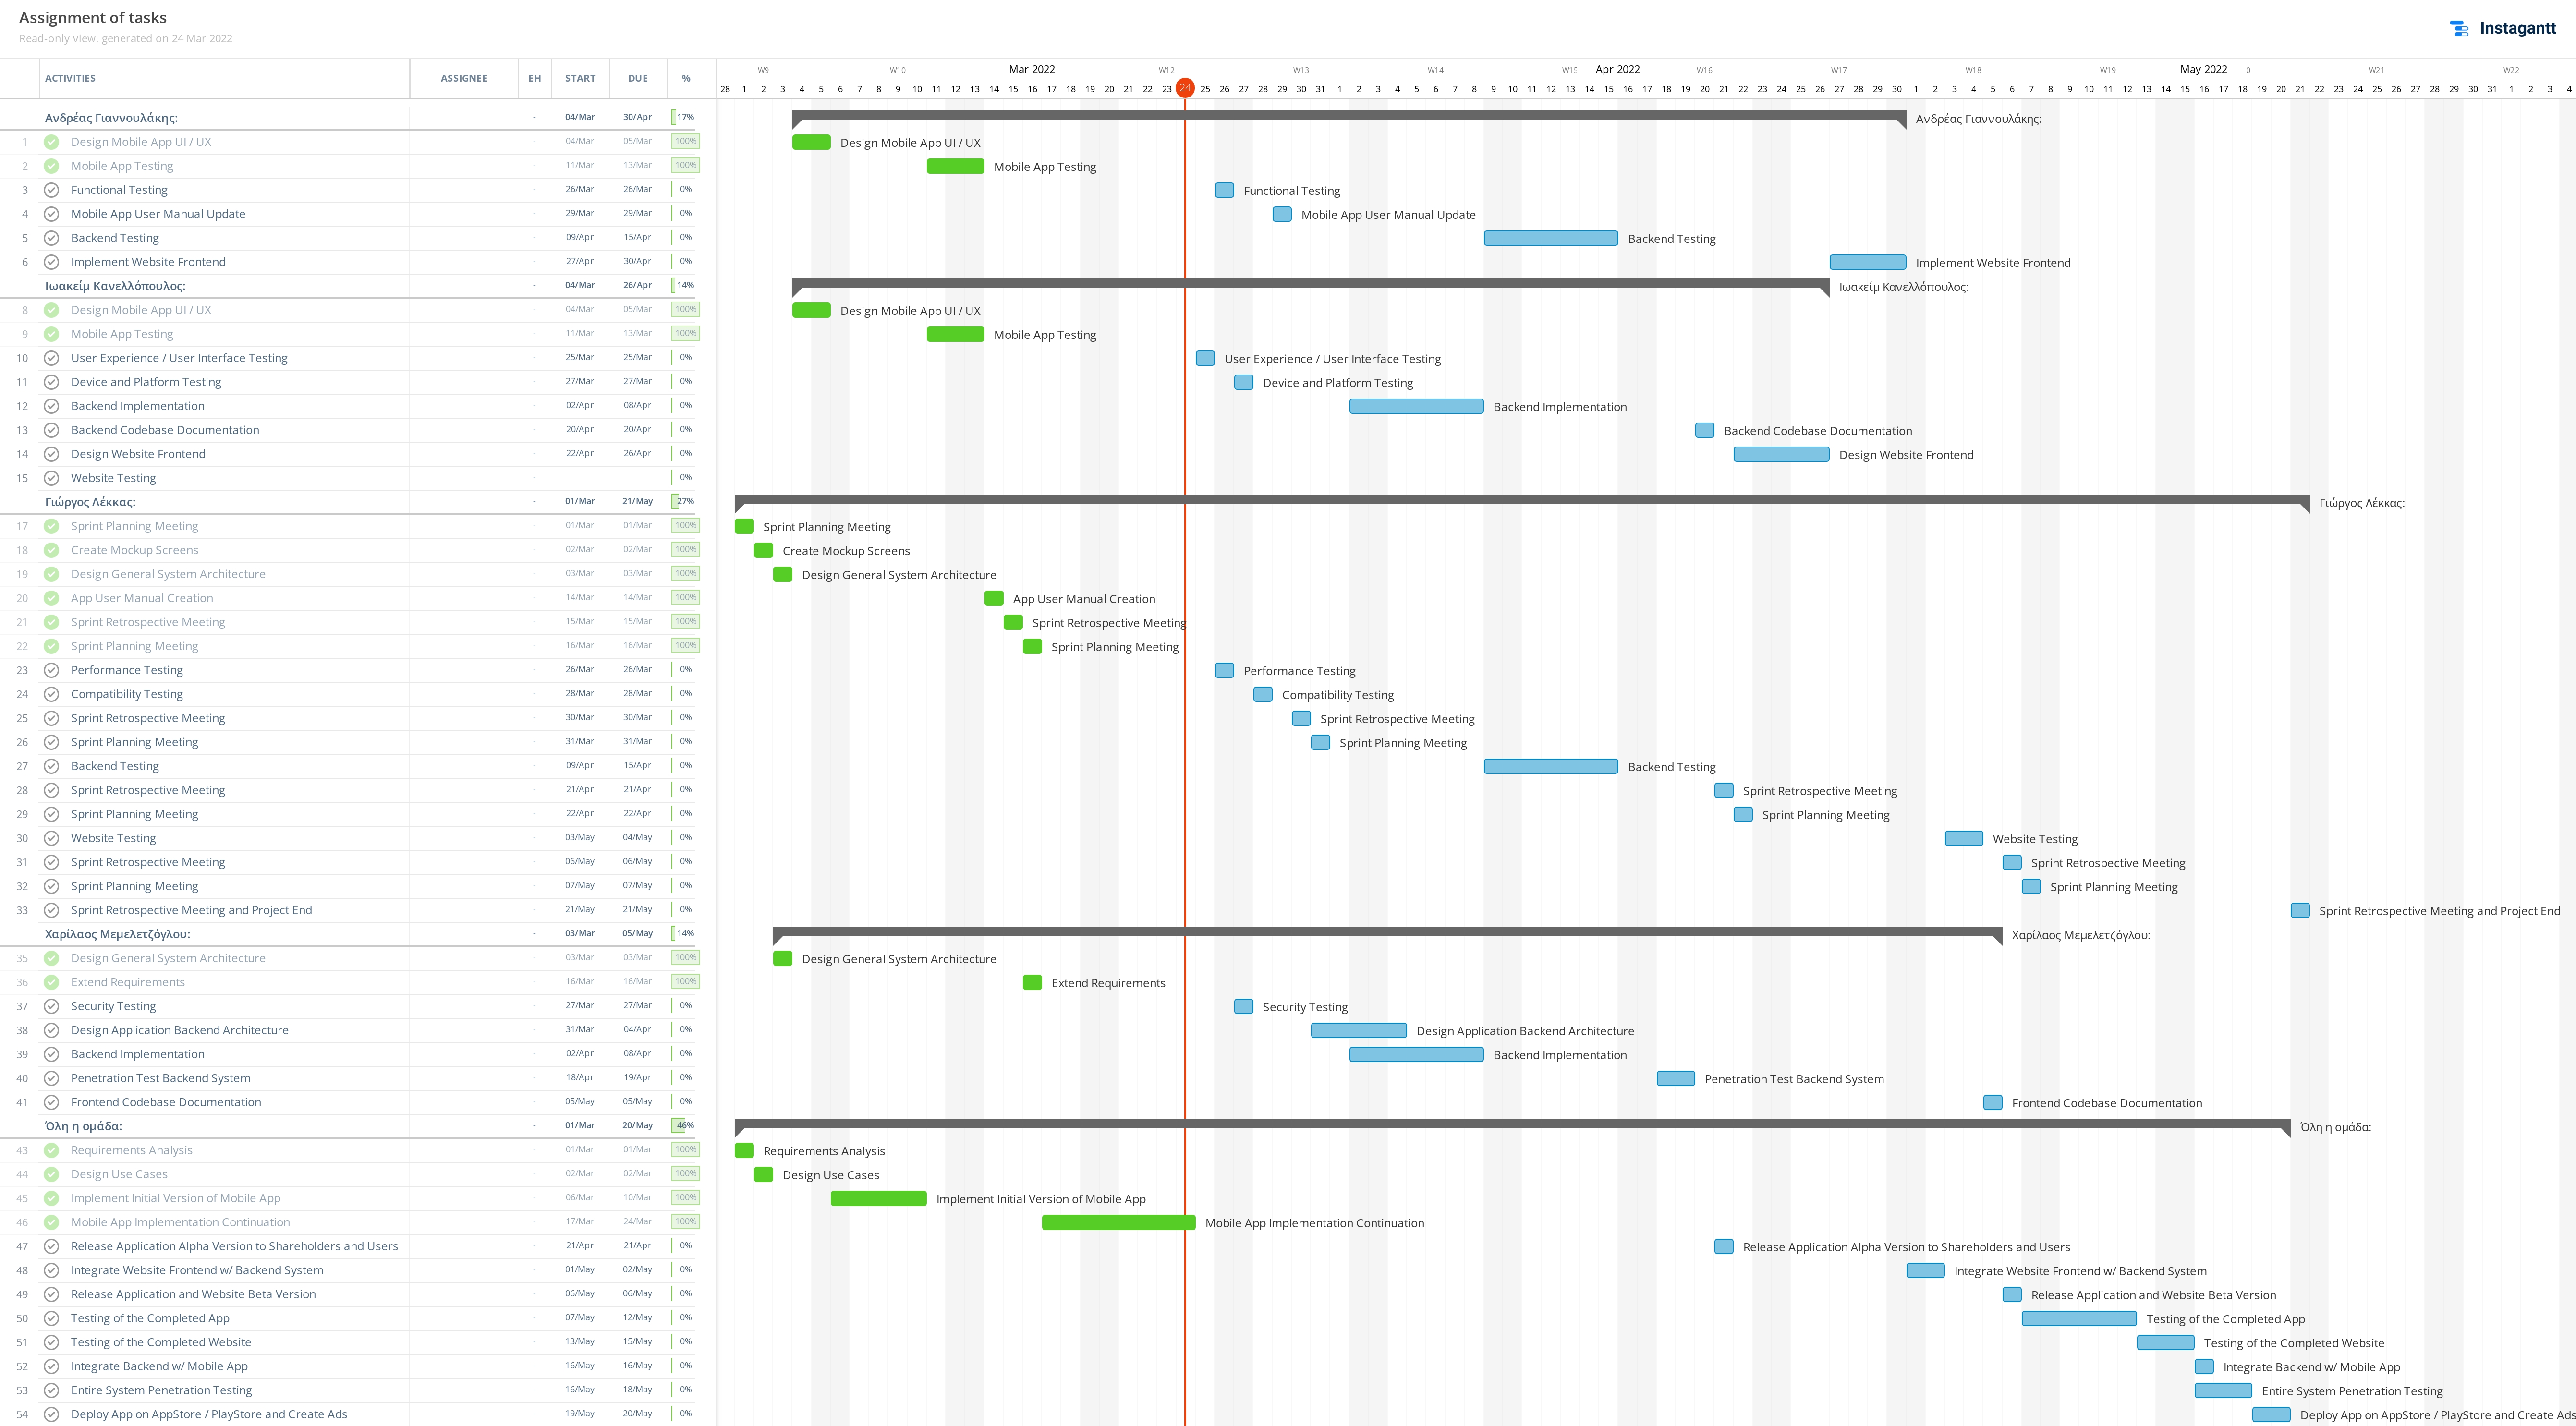
\includegraphics[width=\textwidth, height=\textheight, keepaspectratio ]{img/Ανάθεση_εργασιών.jpg}
		\caption{ \en Gantt Chart \gr Ανθρώπινου δυναμικού}
	\end{figure}
	
	\vspace{20pt}
	\flushleft	
	Επίσης παρακάτω παρουσιάζεται σε μορφή πίνακα η ανάθεση των παραπάνω  \en tasks \gr στα μέλη της ομάδας.	
	
	
	\begin{longtable}{| p{.80\textwidth} | p{.30\textwidth} |} 
		\hline
		\en Sprint Planning meeting \gr & Λέκκας Γ. \\ 
		\hline
		\en Sprint Retrospective Meeting \gr & Λέκκας Γ.    \\ 
		\hline
		\en Requirements Analysis \gr & Όλη η ομάδα    \\ 
		\hline
		\en Design Use Cases \gr    &      Όλη η ομάδα     \\
		\hline
		\en Create Mockup Screens  \gr      &   Λέκκας Γ.        \\
		\hline
		\en Design General System Architecture \gr       &  Μεμελετζόγλου Χ. και Λέκκας Γ.         \\
		\hline
		\en Design Mobile App UI / UX \gr       &  Κανελλόπουλος Ι. και Γιαννουλάκης Α.         \\
		\hline
		\en Implement Initial version of Mobile App \gr       &  Όλη η ομάδα         \\
		\hline
		\en Mobile App Testing \gr       &  Κανελλόπουλος Ι. και Γιαννουλάκης Α.         \\
		\hline
		\en App User Manual Creation \gr       &  Λέκκας Γ.         \\
		\hline
		\en Extend Requirements \gr       &  Μεμελετζόγλου Χ.         \\
		\hline
		\en Mobile App Implementation Continuation \gr       &  Όλη η ομάδα         \\
		\hline
		\en User Experience / User Interface Testing \gr       &  Κανελλόπουλος Ι.         \\
		\hline
		\en Functional Testing \gr       &  Γιαννουλάκης Α.         \\
		\hline
		\en Performance Testing \gr       &  Λέκκας Γ.         \\
		\hline
		\en Security Testing \gr       &  Μεμελετζόγλου Χ.         \\
		\hline
		\en Device and Platform Testing \gr       &  Κανελλόπουλος Ι.         \\
		\hline
		\en Compatibility Testing \gr       &  Λέκκας Γ.         \\
		\hline
		\en Mobile App User Manual Update \gr       &  Γιαννουλάκης Α.         \\
		\hline
		\en Design Application Backend Architecture \gr       & Μεμελετζόγλου Χ.         \\
		\hline
		\en Backend Implementation \gr       &  Κανελλόπουλος Ι. και Μεμελετζόγλου Χ.         \\
		\hline
		\en Backend Testing \gr       & Λέκκας Γ. και Γιαννουλάκης Α.       \\
		\hline
		\en Integrate Backend w/ Mobile App \gr       &  Όλη η ομάδα         \\
		\hline
		\en Penetration Test Backend System \gr       &  Μεμελετζόγλου Χ.        \\
		\hline
		\en Backend codebase documentation \gr       &  Κανελλόπουλος Ι.        \\
		\hline
		\en Release Application Alpha Version to shareholders and Users \gr       &  Όλη η ομάδα        \\
		\hline
		\en Design Website Frontend \gr       &  Κανελλόπουλος Ι.        \\
		\hline
		\en Implement Website Frontend \gr       &  Γιαννουλάκης Α.        \\
		\hline
		\en Integrate Website Frontend w/ Backend System \gr       &  Όλη η ομάδα        \\
		\hline
		\en Website Testing \gr       &  Λέκκας Γ. και Κανελλόπουλος Ι.       \\
		\hline
		\en Frontend Codebase documentation \gr       &  Μεμελετζόγλου Χ.       \\
		\hline
		\en Release Application and Website Beta Version \gr       &  Όλη η ομάδα        \\
		\hline
		\en Testing of the completed App \gr       &  Όλη η ομάδα        \\
		\hline
		\en Testing of the completed Website \gr       &   Όλη η ομάδα        \\
		\hline
		\en Entire System Penetration Testing \gr       &   Όλη η ομάδα        \\
		\hline
		\en Deploy App on AppStore / PlayStore and create Ads \gr       &   Όλη η ομάδα       \\
		\hline
		\en Sprint Retrospective Meeting and Project End \gr       &  Λέκκας Γ.        \\
		\hline
	\end{longtable}
	
	\vspace{30pt}
	
	\newpage
	
	\center{\textbf{Εκτίμηση κόστους του έργου}}
	
	\vspace{20pt}
	
	\flushleft
	Ως εκτίμηση κόστους του έργου θα ληφθεί υπόψη το κεφάλαιο που μπορεί να δαπανήσει η ομάδα ώστε να ολοκληρώσει το έργο σύμφωνα με τις προδιαγραφές που έχει θέσει αλλά και τα πιθανά και αναμενόμενα κέρδη που αναμένεται να αποφέρει η εργασία της ομάδας. Συνεπώς, είναι απαραίτητο να γίνει ένας υπολογισμός των εξόδων και μία λογική εκτίμηση των αναμενόμενων κερδών του \en Project.\gr \\
	
	\vspace{10pt}
	
	
	Η διάρκεια του πρότζεκτ έχει αποφασιστεί να είναι ίση με 3 μήνες.
	
	\vspace{10pt}
	
	Σημείωση : Τα παρακάτω κόστη αποτελούν \textit{εκτίμηση} των συντακτών, και δεν αντικατοπτρίζουν απαραίτητα τα πραγματικά κόστη της ανάπτυξης ενός έργου λογισμικού. \\
	
	\vspace{10pt}
	
	
	Άμεσα κόστη:
	
	\begin{itemize}
		\item Μισθοί Εργατικού Δυναμικού : Έστω ότι ο μέσος μισθός των \en developers \gr στην Ελλάδα, είναι ίσος με 1500 €. Η ομάδα μας αποτελείται από 4 άτομα, η διάρκεια του \en Project \gr είναι ίση με 3 μήνες, άρα συνολικό κόστος : \textit{1500 Ευρώ/Μήνα * 3 Μήνες * 4 Μέλη  } = \textbf{18.000 €} 
		
		\item Κόστος δημοσίευσης εφαρμογής :100 € (\en Apple AppStore), 20 €(Google PlayStore)  \gr. Συνολικό κόστος = \textbf{120 €}.
		
		\item Συντήρηση Εφαρμογής: \textbf{150 €} ανά 3 Μήνες, αφού η εφαρμογή δημοσιευθεί.
		
		\item Κόστος χρήσης Χάρτεων και Τοποθεσίας (\en Geolocation API\gr) : \textbf{90 €}  για 3 Μήνες
	\end{itemize}
	
	Άθροισμα Αρχικών Άμεσων Κοστών = \textbf{18.210 €} + 150 €/Μήνα για την συντήρηση της εφαρμογής.
	
	\vspace{20pt}
	
	'Εμμεσα Κόστη:
	
	\begin{itemize}
		\item Σύνδεση στο \en Internet \gr : \textbf{60 €} για 3 Μήνες
		\item Ενοικίαση χώρου εργασίας : \textit{800 € * 3 Μήνες} = \textbf{2400 €}
		\item Λειτουργικά έξοδα χώρου εργασίας (Ρεύμα, Νερό, κλπ) : \textit{200 €/Μήνα * 3 Μήνες} = \textbf{600 €}. 
		\item Πιθανά νομικά έξοδα: \textbf{1200€}
		\item Διαφημιστική Εκστρατεία (\en Marketing Campaign \gr) : \textit{150 €/Μήνα * 3 Μήνες} = \textbf{450 €}.
	\end{itemize}
	
	Άθροισμα Άμεσων Κοστών = \textbf{4.710 €}
	
	\vspace{20pt}
	
	\textbf{Συνολικό κόστος έργου: 22.920€ } + 150 €/Μήνα για την συντήρηση της εφαρμογής.
	
	\vspace{20pt}
	
	
	Εκτιμώμενα Κέρδη:
	
	\begin{itemize}
		\item Κέρδη απο διαφημίσεις εντός της εφαρμογής : \textbf{300 €/Μήνα}.
		\item Ενεργοποίηση \en Premium \gr έκδοσης για αφαίρεση διαφημίσεων : \textbf{5 €/ενεργοποίηση}
		
		\item 'Εσοδα από την συμφωνία πώλησης της εφαρμογής, στην πολυεθνική εταιρία (πελάτης της ομάδας) : \textbf{30.000 €} (αγνοώντας του φόρους).
		
		Συνεπώς, αναμένουμε κέρδος \textbf{7.500 €/άτομο} .
		
	\end{itemize}
	
	
	
\end{document}
